\documentclass[usenatbib]{mnras}
\usepackage{siunitx}
\usepackage{graphicx}	% Including figure files
\usepackage[utf8]{inputenc}
\usepackage[english]{babel}
\usepackage{float}
\usepackage{amssymb, amsmath, yhmath}
\usepackage{verbatim}

\newcommand{\expect}[2]{\left< #1 \right| #2 \left| #1 \right>}
\renewcommand{\d}[1]{\! \mathrm{d}#1 \:}
\newcommand{\deriv}[2]{\frac{\d{#1}}{\d{#2}}}
\newcommand{\pderiv}[2]{\frac{\partial{#1}}{\partial{#2}}}
\newcommand{\parsq}[2]{\frac{\partial^2{#1}}{\partial{#2}^2}}


\bibliographystyle{apa}
\setlength{\bibhang}{1in}
\setcitestyle{authoryear, open={(},close={)}}
\renewcommand{\bibsection}{\section*{References}}

\usepackage{graphicx}

\newcommand{\squote}[1]{\lq #1\rq}

\renewcommand{\d}[1]{\ensuremath{\operatorname{d}\!{#1}}}
\newcommand{\poweV}[1]{\SI{e#1}{\electronvolt}}
\newcommand{\ineV}[2]{\SI{#1 e #2}{\electronvolt}}
\newcommand{\lcdm}{$\Lambda$CDM}
\DeclareSIUnit\parsec{pc}
\DeclareSIUnit\lightyear{ly}
\DeclareSIUnit\year{yr}
\begin{document}

\title[Dark Matter Heating]{Heating of Milky Way Disk Stars by Dark Matter Fluctuations in Cold Dark Matter and Fuzzy Dark Matter Paradigms}
\author[B. V. Church and J. P. Ostriker]{
Benjamin V. Church$^{1}$ \thanks{Contact e-mail: bvc2105@columbia.edu}, Philip Mocz$^{2}$ \thanks{Einstein Fellow},
Jeremiah P. Ostriker$^{1}$ \thanks{Contact e-mail: jpo@astro.columbia.edu}
\\
$^{1}$Columbia University, Department of Astronomy, New York, NY 10025, USA.
\\
$^{2}$Department of Astrophysical Sciences, Princeton University, 4 Ivy Lane, Princeton, NJ, 08544, USA.}
\maketitle
\begin{abstract}
Although highly successful on cosmological scales, Cold Dark Matter (CDM) models predict unobserved over-dense \squote{cusps} in dwarf galaxies and overestimate their formation rate. We consider an ultra-light axion-like scalar boson which promises to reduce these observational discrepancies at galactic scales. The model, known as Fuzzy Dark Matter (FDM), avoids cusps, suppresses small-scale power, and delays galaxy formation via macroscopic quantum pressure. We compare the substructure of galactic dark matter halos comprised of ultra-light axions with masses $\poweV{-24} \leq m_p \leq \poweV{-18}$ to conventional CDM results. Besides self-gravitating subhalos, FDM includes additional substructure in the form of non-virialized over-dense wavelets formed by quantum interference patterns. Wavelets provide a more efficient source of heating to the central galactic disk than do subhalos. We provide analytical measures of substructure-induced perturbations and heating to interior test particles responsible for the thickening of galactic disks. FDM models can produce a cumulative heating of $30\, \si{\kilo\meter\per\second}$ over an approximate galaxy lifetime of $10\, \si{\giga\year}$ which corresponds to the velocity dispersion of the Milky Way thick disk. We provide explicit calculations of the radial dependent disk velocity dispersion and corresponding scale height. Although the source of thickened disks is not known with any certainty, the heating due to perturbations caused by dark substructure cannot exceed the total disk velocity dispersion. This work provides a lower bound on the FDM particle mass $m_p > 1.27 \times \SI{e-22}{\electronvolt}$. FDM wavelets should be considered a viable mechanism for producing the observed disk thickening. 
\end{abstract}

\begin{keywords}
cosmology: theory -- dark matter -- galaxies: structure
\end{keywords}

\section{Introduction}

The dark sector contributes a sizable majority of all matter in the universe. The existence of one or more kinds of dark matter is essential to galaxy formation and consistency with observed disk rotation curves. Over-dense regions of dark matter collapse to roughly localized concentrations of matter called ‘halos’ which are well-described by approximately spherically symmetric density profiles \citep{structure}. However, computationally identical halos may vary significantly from these profiles in small-scale power i.e. substructure. Various models for the underlying physics of dark matter predict various patterns of density irregularities which, though invisible to the electromagnetic spectrum, are capable of perturbing the orbits of stars via gravitational effects. We will attempt to estimate those effects on the observable stars in galactic disks to better constrain our understanding of the fundamental nature of the dark matter.
             
\par 

The standard cosmological model (\lcdm) contains a massive electromagnetically non-interacting component known as Cold Dark Matter (CDM) with density parameter $\Omega_c = 0.259 \pm 0.006$ \citep{planck}. The properties of this substance are largely unknown and are assumed to be approximately that of a perfect fluid with negligible pressure compared to its energy density i.e. comprised of cold or non-relativistic matter at high redshift. CDM simulations suggest that substructure forms self-gravitating clumps which are qualitatively similar to free dark matter halos. We adopt a substructure formalism which tracks subhalos as an estimate of total substructure. The secondary gravitational effects of these subhalos is dependent on the subhalo mass function and the shape of small halo profiles, which is directly dependent on properties of the dark matter physics under consideration. Constraints obtained from The Sloan Digital Sky Survey measurement of Ly-$\alpha$ forest power spectra and surveys of dwarf galaxies below the free-streaming scale rule out most models of relativistic (hot) matter as the primary component of dark matter \citep{can_neutrinos}. Attempts to directly detect CDM particles in various plausible models of physics beyond the standard model have so far been without success \citep{direct_detection}.
	  
\par

Although amazingly accurate on cosmological scales, CDM models fail to make accurate predictions when compared with observations at distance scales less then \SI{1}{\kilo\parsec}. When compared with studies of dwarf galaxy rotation curves, CDM predicts unobserved density \squote{cusps} in the center of dark matter halos \citep{ultralight}. This failure is known as the \squote{cusp-core problem}. Another serious concern is the \squote{missing satellite problem}  \citep{missing_satellites}. The number of satellite galaxies predicted for a milky-way-like galaxy is greater than what we observe by an order of magnitude. This issue is sharpened by the \squote{too big to fail} problem of galaxy formation that claims some of the predicted satellites are so massive that it is difficult to imagine that they would not form any stars \citep{too_big_to_fail}. Various complex phenomena have been suggested as solutions to these problems such as baryonic feedback mechanisms which redistribute matter or  hypothetical dark matter self-interactions.

\par

An alternative model gaining popularity known as Fuzzy Dark Matter (FDM) characterizes the bulk of dark matter as comprised of ultra-light($m \approx \poweV{-22}$) bosons whose characteristic de Broglie wavelength is on the order of $\SI{1}{\kilo\parsec}$. Such ultra-light particles are possible in various theories beyond the standard model \citep{axion_cosmology}. In particular, the class of axion-like particles is a perfect candidate for FDM and therefore, we refer to the mass of the constituent particles of FDM as the axion mass $m_p$. Macroscopic quantum mechanical wave effects “smear” the density profile on scales less than $\sim \SI{1}{\kilo\parsec}$ which removes problematic cusps from the center of large halos. These cusps are replaced by dense self-gravitating quantum states known as soliton cores which may facilitate indirect observational evidence for FDM. Furthermore, the quantum mechanical pressure caused by the large wavelength of FDM suppresses the formation of low-mass halos and entirely eliminates the formation of any halo or subhalo smaller than this wavelength, reducing or eliminating the missing satellites problem \citep{substructure_FDM}. Significant further effort remains in determining further discrepancies between FDM and CDM and whether these can, in conjunction with observational constraints, rule out one or both of the models.
 
\par

The dynamical effects of CDM have been studied in some detail, especially regarding the accretion and tidal stripping of CDM subhalos by large galaxies and their associated dark matter halos. On the other hand, research on the dynamics of FDM distributions is developing rapidly (c.f. \cite{schive_solitons, Schrodinger-Poisson, Schive-virialized-wave-halos}) but still in its infancy. However, dynamical studies have focused on simulations which inherently have a fixed resolution and thus are limited to small (approximately \SI{1}{\mega \parsec} scales) cosmological volumes and low ($M < 10^{12} M_{\odot}$) halo masses. In this paper, we present analytic estimates for substructure dynamical fluctuations which do not suffer from limited resolution. The resolution limit of simulations causes underestimates to subhalo populations and therefore to their dynamical effects. 
\par 
	CDM and FDM models predict significant differences in the distribution of halo substructure. While CDM predicts a power law divergence in the number of small subhalos, the FDM subhalo mass function is zero below a cutoff scale determined by the axion mass expressed by the Jean’s scale at which quantum pressure and gravitational attraction balance:
\setlength{\belowdisplayskip}{4pt} \setlength{\belowdisplayshortskip}{4pt}
\setlength{\abovedisplayskip}{4pt} \setlength{\abovedisplayshortskip}{4pt}

\begin{equation}
k_J = 66.5 \cdot (1+z)^{1/4} \left( \frac{\Omega_a h^2}{0.12} \right) \left(\frac{m_p}{\poweV{-22}} \right)^{1/2} \si{\per\mega\parsec}
\end{equation}
\noindent
as given by \citet{axion_cosmology}. \\ For ultra-light axions, the subhalo mass function is significantly suppressed though the entire range of substructure for a halo comparable to the Milky Way’s. However, FDM subhalos will exhibit solitons which, for moderately-sized subhalos and large axion masses, are very dense and largely unaffected by tidal disruption. The main deviation from CDM phenomena occurs on scales smaller than the coherence length. Above this scale, the Schr\"{o}dinger-Poisson–Vlasov-Poisson correspondence predicts that the self-gravitating nonlinear Schr\"{o}dinger equation governing FDM reproduces the physics of collisionless particulate dark matter \citep{Schrodinger-Poisson}. Simulations using zoom-in techniques are able to resolve complex structure in the core of an FDM halo and have discovered large-amplitude oscillations in the core density of such halos \citep{structure-FDM-halos}. In addition, a surprising standing wave phenomenon has been observed in the density profiles produced by small-scale FDM computer simulations \citep{cold_and_fuzzy}. These standing waves, named wavelets, radically alter the dark matter profile and may, through gravitational interactions, disturb the baryonic components in directly measurable ways. The primary effect of these wavelets is to introduce time-varying perturbations to the gravitational potential on a much shorter time-scale than the evolution of primary structure after the system has come into virial equilibrium \citep{Schrodinger-Poisson}. 
\par
	The velocity dispersion of stars in a galactic disk provides a proxy to study the gravitational perturbations produced by the dark matter halo substructure. We know that the dispersion increases with age via an approximate power law $\sigma \propto t^\beta$ \citep{heating_history}. Therefore, the best observational bounds will come from old, thick disk stars.  

\section{Galactic Disks}

\hspace{5mm} Current observations suggest that the disks of spiral galaxies may be roughly modeled by an approximately exponential profile in radius and in vertical structure. The vertical scaling is determined by the mass density of the disk and the perpendicular velocity dispersion.  The bulk of the stars in normal disks are divided into a thin disk of relatively young stars and a thick disk of old stars \citep{binney_tremaine_2008}.  The velocity dispersion of the old stars is significantly greater which is why this population is referred to as the thick disk. Thick disk stars show reduced metallicity which suggests they originate from an earlier epoch of star formation than the thin disk stars \citep{binney_tremaine_2008}. 
\par
Studies of the velocity dispersion of Milky Way stars at varying angles and scale heights showed that the velocity dispersion of the thick disk is time dependent and fit approximately by a power law $\sigma_D \propto t^{\beta}$ where the best estimates for the exponent are $\beta \approx 0.3$ \citep{heating_history}. The origin of this twin disk structure is unknown but there are three widely considered explanations. One hypothesis is that the thick disk formed with subsequent stellar generations born in ever slimmer disks due to energy loss of the disk to gas shocks. However, this explanation struggles to explain the observed decrease in velocity dispersion with redshift \citep{emergence-thick-disk}. An alternative hypothesis is that tidal interactions between galaxy close encounters can inject energy into existing stars which effectively puffs up the disk \citep{thick-disk-mergers}. A final possibility is that the thick disk is formed by continually heating older stars \citep{thin-and-thick-disk}. 
\par 
The primary source of heating remains uncertain. Interactions between spiral modes have been proposed as a mechanism for heating spiral disks but the ability to heat up to the velocity dispersion of the old disk stars by spiral modes remains to be demonstrated. Here we will consider the possibility that disk heating is caused by interactions with dynamical dark substructure of the halo. In this case, we will be able to sharply restrict the parameter space of possible dark matter paradigms. Regardless of the origin of thick disks, the heating due to dark substructure can at most account for the total observed velocity dispersion of the thick disk. Therefore, these results are able to put a lower bound on the mass of the FDM axion which is agnostic to the mechanism behind producing thick disks.
\par
The disks of normal spiral galaxies approximatly follow an exponential radial density profile,
\begin{equation}
\rho(r, z) = \frac{\Sigma_0}{2 H(r)} e^{-r/r_0} \mathrm{sech}^2{(z/H(r))} 
\end{equation}
where $r_0$ is the scaling radius and $H(r)$ is the scale height at a given radius. The indicatd vertical dependece is exact only for a disk which is isothermal along vertical slices of constant radius. Furthermore, the projection of the mass density onto the galactic plane has the same exponential form. In particular, the local surface density as a function of radius has approximately the form,
\begin{equation}
\Sigma(r) = \int_{-\infty}^{\infty} \rho(r, z) \d{z} = \Sigma_0 e^{-r / r_0}
\end{equation}
For the Milky Way, these parameters are estimated to be $r_0 = \SI{5}{\kilo \parsec}$ and $\Sigma_0 = \SI{64}{M_{\odot} \per \parsec \squared}$ \citep{dynamical_measurement}. The vertical profile is determined by hydro-static equilibrium under the gravity from the planar density distribution of the disk. The pressure supporting the vertical structure is given by the vertical velocity dispersion $P = \rho \sigma_D^2$. 
\begin{equation}
- 4 \pi G \rho = \frac{\partial^2 \phi}{\partial z^2} = \pderiv{}{z} \left( \frac{1}{\rho} \pderiv{ \rho \sigma_D^2}{z} \right)
\end{equation}  
Therefore, integrating through the disk and approximating $\sigma_D^2$ as varying slowly vertically through the disk we arrive at the following expression relating the scale height and vertical velocity dispersion of the disk.
\begin{equation} \label{scale}
4 \pi G \Sigma(r) = \frac{ \sigma_D(r)^2 }{H(r)}
\end{equation}
For stars oscillating through the disk with vertical displacement large compared to the scale height the period of oscillation is simply given by approximating the the disk gravity as producing a constant magnitude restoring force. Therefore the period for a star with vertical velocity $\sigma_D$ is given approximately by,
\begin{equation}
P = \frac{2 H}{\sigma_D} = \frac{2 \sigma_D}{4 \pi G \Sigma}
\end{equation}
The period of disk oscillations determines the adiabatic cutoff for heating due to perturbing interactions. Under the assumption that disk thickening is due primarily to the proposed dark substructure dynamics, the dependence on radius of the disk velocity dispersion $\sigma_D$ can be calculated explicitly. Using the above relations and the radial dependence of $\sigma_D$ we will be able to predict the radial thickness profile of the galactic disk and compare these results to measurements of the flaring of actual disks.  
\par
We now turn our attention to the Milky Way which has the best studied galactic disk. \cite{milky_way} has performed a comprehensive study of the various distribution functions of the Milky Way and, in particular, has compiled data on the velocity dispersion of the thin and thick disks as a function of vertical distance. \cite{milky_way} proposes a ``pseudo-isothermal'' distribution function for the velocity dispersion which has the form,
\begin{equation}
f_z(J_z) = \frac{\left( \Omega_z J_z + V_\gamma^2 \right)^{-\gamma}}{2 \pi \int_{0}^{\infty} \d{J_z} \: \left( \Omega_z J_z + V_\gamma^2 \right)^{-\gamma} }
\end{equation}  
in term of the action variable $J_z$. For stars in the solar neighborhood with $r \approx R_0 =  \SI{8}{\kilo \parsec}$ the best fit parameters of $\gamma = 2.6$ and $V_\gamma = \SI{18.7}{\kilo \meter \per \second}$ give excellent agreement with survey data collected by \cite{milkyway-thickdisk}. Using this formalism, the main component of the perpendicular velocity dispersion of the thick disk is $\sigma_D \approx \SI{34}{\kilo \meter \per \second}$ at the solar neighborhood near the radius $R_0$.   



\section{Heating via Substructure Dynamics}

We provide models for how dynamical halo substructure can heat galactic disks due to time-varying gravitational interactions. First we will consider self-gravitating substructure in both CDM and FDM of which the dominant form is approximately self-similar subhalos. Additionally, we will consider the peculiar feature of wave dark matter which produces time-dependent substructure on the order of the de Broglie wavelength due to interference. This wavelet substructure provides an additional source of heating which is qualitatively very different from the heating due to subhalos because the wavelets are not self-gravitating objects. 

\subsection{Estimating The Heating Due to Transits}

We first provide a rough analysis of the heating due to transiting over-dense regions of dark matter. Each transit causes a change in velocity of approximately,
\begin{equation}
\Delta v^2 = \frac{M_l G}{b v_l}
\end{equation}
where $M_l$ is the mass of the region, $v_l$ is its velocity, and $b$ is the distance at closest approach. However, the heating is ineffective if these perturbations are adiabatic which will merely cause gradual periodic changes rather than overall heating to the orbits whose adiabatic invariants remain fixed. However, if the heating is roughly impulsive then the orbits will be irreversibly perturbed. The non-adiabatic condition approximately corresponds to the constraint,
\begin{equation} \label{adiabatic}
\frac{b}{v_l} < \frac{P}{2}
\end{equation}
where $P$ is the characteristic period of the objects subjected to perturbation, in this case the period for lateral oscillations through the galactic disk. The heating of the disk is measured by tracking the one-dimensional velocity dispersion of the disk $\sigma_D^2 = \left< \dot{z}^2 \right>$ over time. The total rate of heating is therefore given by the accumulation of all such encounters,
\begin{subequations}
\begin{align}
\deriv{\sigma_D^2}{t} &= \int (2 \pi b) \: \d{b} \: n v_p \: \left( \frac{M_l G}{b v_p} \right)^2 
\\
& = \frac{M_l^2 G^2}{v_l} \: 2 \pi n \ln{\Lambda}
\end{align}
\end{subequations}
where we have defined,
\begin{equation}
\ln{\Lambda} := \ln{\left( \frac{b_{\text{max}}}{b_{\text{min}}} \right)}
\end{equation}
which is the gravitational equivalent of the Coulomb logarithm. Here $v_l$ is the relative velocity between the disk and the perturbing objects in the halo. 
The maximum distance across which the heating is efficient is fixed by equation \eqref{adiabatic} and the minimum distance is given by $r_l$, the characteristic size for the perturbing objects. Furthermore, the period of oscillation out of a thin disk is given by the velocity dispersion and surface density of the disk via,
\begin{equation}
P = \frac{2 \sigma_D}{4 \pi G \Sigma}
\end{equation} 
Therefore, in terms of the overall one-dimensional velocity dispersion, we derive the time-dependent heating as,
\begin{subequations}
\begin{align}
\deriv{\sigma_D^2}{t} &= \frac{M_l^2 G^2}{\sigma_H} \: 2 \pi n \ln{\Lambda}
\\
\Lambda & = \frac{\sigma_H \sigma_D}{4 \pi G \Sigma \: r_l}
\end{align}
\end{subequations}
A more detailed calculation found in \cite{milkywayblackholes} gives somewhat altered numerical factors,
\begin{align} \label{heating}
\deriv{\sigma_D^2}{t} = \frac{8 \pi M_l^2 G^2}{\sqrt{2} \sigma_H} \: n \: \ln{\Lambda}
\end{align}
We define the quantity,
\[ \sigma_{10} = \left( \deriv{\sigma_D^2}{t} \cdot (\SI{10}{\giga \year}) \right)^{1/2} \]
as a standard measure of the approximate heat over an estimate of the age of a Milky Way-like halo.
\par
	An alternative approach for calculating heating due to transits is given by \cite{ultralight} which only considers the tidal effects on disk heating. That model assumes that only local dispersion with acting across a characteristic scale much smaller than $H$ can lead to overall heating. However if processes such as outgoing density waves are an inefficient means for dissipating differential motions of the disk then dynamical friction between oscillating disk components will tend to dissipate oscillation energy into disk heating and therefore contribute to the thickening. In this analysis, we will assume that such processes are inefficient and therefore equation \eqref{heating} gives a more reasonable estimate of the total rate of disk heating.  
	
	
The calculation we provide is based on the total kinetic energy delivered into vertical motions of the disk. These motions can be broken ino two components: those reflecting a direct increase in the z-velocity dispersion and those invested in bending waves which give one part of the disk a z-velocity with respect to the mean disk velocity. Some fraction of the second component could be damped by transfer of energy back to the dark matter, to gas motions, or be tranfered radially outwards in propagating bending disk waves. Thus, our calculation provides an upper bound on the disk heating by subhalos and wavelets with the calculation given by equation (37) of \cite{ultralight} giving a lower bound.   	

\subsection{Heating Due to Subhalos}

\subsubsection{Spatial Profile}

	We model substructure as comprised entirely of subhalos which act as distinct massive particles subject only to gravitational attraction and tidal disruption. Following \citet{tidal_limit} and \cite{unified_model} we adopt a
simplified model of subhalo
formation and dynamics. The initial shape of
the subhalo mass function is assumed to
be spatially invariant, i.e. the position
and mass variables are decoupled. The
total density of subhalos is assumed to
follow the Navarro--Frenk--White (NFW) profile:
\begin{equation}
\rho(r) = \frac{\rho_0}{r/r_c (1+r/r_c)^2}
\end{equation} which also
describes the density profile of the
primary dark matter halo given by \citet{structure} from CDM simulations. This profile is fairly universal for the halos of massive cold particles which we assume accurately describe subhalos. Furthermore, we are working under the assumption that the primary modifications of subhalos relative to free halos arise from tidal stripping. Wave dark matter models modify the primary halo density profile away from NFW. However, the core behavior is primarily due to quantum pressure which does not act between self-gravitating lumps. Therefore, we do not expect the spatial distribution of subhalo formation to be significantly altered from FDM. That said, due to extreme tidal disruption, subhalos near the core of the primary halo contribute negligibly, so the exact shape of their distribution near the core is unimportant.  

\subsubsection{The Subhalo Mass Function}

The only additional information needed to calculate the perturbations due to subhalos is the distribution of subhalo populations as a function of mass. However, the tidal interactions between the primary halo and its interior subhalos complicates the elegant halo mass functions determined by the over-density correlation function and power spectrum. We approximate the subhalo populations by assuming that the unresolved subhalo mass function has the same form as the free halo mass function derived from the extended Press--Schechter formalism. The unresolved mass function is then modified by tidally truncating unresolved halos such that the unresolved halo mass function is shifted towards lower mass and the modified subhalo mass function becomes coupled in subhalo mass and radius inside the primary halo. Therefore, the population of subhalos is entirely determined by two functions, $\frac{\d{n}}{\d{\ln{M}}}$, the unresolved (free) halo mass function, and $T_R(M)$, the truncated mass function at a radius $R$.

\subsubsection{Calculating the Heating}

In terms of these functions the rate of heating is given by,
\begin{equation} \label{subhaloheating}
\deriv{\sigma_D^2}{t} = \frac{8 \pi G^2}{\sqrt{2} \: \sigma_H} \int_0^{M_p} T_R(m)^2  \deriv{n}{m}  \ln{\frac{\sigma_H \sigma_D}{4 \pi G \Sigma \: r_{\text{t}}(m)}} \d{m}
\end{equation}   
where $r_{\text{t}}(m)$ is the radius of a subhalo of mass $m$ after truncation at a radius $R$. 
If we assume that the primary halo and substructure formed quickly on the scale the lifetime of the disk, and that dark substructure dynamics in the form of transiting subhalos alone constitutes the primary source of disk thickening then equation \eqref{subhaloheating} gives the time-dependence of $\sigma_D$ as a function of time over the entire history of the halo. Furthermore, the rate of heating given by equation \eqref{subhaloheating} depends on $\sigma_D$ only logarithmically. Therefore, the square of the velocity dispersion increases with an approximately constant rate analogously to a random walk. Therefore, this heating model predicts an exponent, $\beta \approx \tfrac{1}{2}$ in the time dependence $\sigma_D \propto t^{\beta}$.

\subsection{Heating Due to Quantum Wavelets in FDM}

In models of wave dark matter, there is an added contribution to the fluctuating substructure due to interference of excited modes which produce time dependence over-density known as wavelets. We assume that the density of the wavelets is a fixed multiple of the local mean density. Using results from numerical FDM simulation given by \cite{BECDM},
\begin{equation} \label{mutiple_of_background}
M_w = A \left(\frac{\lambda_{\text{char}}}{2} \right)^3 \rho(r) 
\end{equation}  
where $\lambda$ is the local characteristic scale. Because these wavelets are inherently produced by quantum mechanical interference, they will approximately saturate the uncertainty relations such that,
\begin{equation}
\lambda m_p \sigma_H \approx \hbar
\end{equation}
where $m_p$ is the particle mass. However, the numerical factors in this relationship are important for giving an accurate bound on the particle mass. Therefore, we will provide a more detailed treatment. We also assume that entire mass of the primary FDM halo (external to the central soliton) is in the wavelets such that,
\begin{equation} \label{const}
M_w n = \rho(r)
\end{equation}
These wavelets are characterized by their velocity dispersion 
$\sigma_{\rm D}$.
Although classically, the particles would have an approximately Maxwell-Boltzmann distribution:
\begin{equation}
f(\mathbf{v}) \propto \exp\left(-v^2/(2\sigma_{\rm D}^2/3)\right)
\end{equation}
quantum mechanically, by the Schr\"{o}dinger-Poisson–Vlasov-Poisson correspondence, the wave function is given by:
\begin{equation} \label{phase_dist}
\psi(\mathbf{x}) \propto \sum_{\mathbf{v}} f(\mathbf{x},\mathbf{v})^{\frac{1}{2}} \exp{\left[i m \mathbf{x}\cdot\mathbf{v}/\hbar + 2\pi i \phi_{{\rm rand},\mathbf{v}} \right]}
\, \mathrm{d}^{3}{\mathbf{v}}
\end{equation}
(equation 27, \cite{Schrodinger-Poisson}) where $\phi_{{\rm rand},\mathbf{v}}\in[0,2\pi)$ is a random phase associated with velocity $\mathbf{v}$.
Such a constructed wavefunction is in agreement with the a local patch of the wavefunction seen in simulated idealized virialized halos \citep{BECDM}.
In such a distribution, structure is totally suppressed below the deBroglie wavelength $\lambda_{\rm dB} \equiv \hbar/(m_p\sigma_D)$ by the uncertainty principle.
The characteristic size of these wavelets (seen numerically in the peak of the density power spectrum) is a multiple of the suppression scale:
\begin{equation} \label{characteristic_wavelength}
\lambda_{\text{char}} = \frac{ 2 \pi \hbar}{m_p \sigma_H \sqrt{\frac{3}{2}}} 
\end{equation}
Using equation \eqref{mutiple_of_background}
and also the constraint of equation \eqref{const} then numerically, for a distribution given by equation \eqref{phase_dist}, counting the number of peaks per unit volume $n$, we find $A\simeq 2.2$.
Therefore, the heating due to wavelets is approximately given by,
\begin{subequations} \label{FDMheating}
\begin{align}
\deriv{\sigma_D^2}{t} & = \frac{2 \pi A}{3 \sqrt{3}} \left( \frac{2 \pi \hbar }{m_p} \right)^3 \frac{(\rho(r) G)^2}{\sigma_H^4} \ln{\Lambda}
\\
\Lambda & = \frac{m_p\sigma_H^2 \sigma_D}{4 \pi \hbar G \Sigma}
\end{align}
\end{subequations}
Therefore, using $\Sigma = \Sigma_0 e^{-r/r_0}$ we can express the rate of heating as a function of radius. The Schr\"{o}dinger - Poisson equations which govern the dynamics of a self-gravitating quantum superfluid (such as FDM) exhibit a general scaling symmetry:
\begin{equation}
\{ x, t , \rho, m \} \to \{\alpha x, \beta t, \beta^{-1} \rho, \alpha^{-2} \beta m \} 
\end{equation}
\noindent \citep{Schrodinger-Poisson}.
We find that equation \eqref{FDMheating} is consistent with this general scaling relation. Under the same assumptions that the considered dynamics are the dominant contribution to disk thickening, as before, the rate of heating given by equation \eqref{subhaloheating} depends on $\sigma_D$ only logarithmically. Therefore, the square of the velocity dispersion increases with an approximately constant rate analogously to a random walk. This heating model also predicts an exponent, $\beta \approx \tfrac{1}{2}$ in the time dependence $\sigma_D \propto t^{\beta}$. Once again we note that, since we are considering both components of disk heating as ultimately being reflected in the z-velocity dispersion, we here provide an upper bound on the effect. 
\subsection{Heating in the CDM Paradigm}

\subsubsection{Unresolved Mass Function}

As the primary halo forms, it captures subhalos via accretion. The unresolved subhalo mass function refers to the distribution of subhalo masses at the time of accretion before dynamical effects such as tidal stripping have biased the distribution. We assume the unresolved subhalo mass function is very close in shape to the free halo mass function truncated above the primary halo mass. Based on simulations given by \citet{dark_wave} we take this fraction to be $\sim 10\%$. The CDM halo mass function and corresponding subhalo mass function calculated from simulations \citep{pop_of_subhalos, unified_model} are well fit by a power law in the accretion mass $m_{acc}$ which denotes the mass of a subhalo before modification by the external tidal field. This form matches the free halo mass function, 
\begin{equation}
\frac{\d{n}}{\d{\: \ln{m_{acc}}}} = C \left(\frac{\rho(r)}{M_p}\right) \left(\frac{m_{acc}}{M_p} \right)^{-p} 
\end{equation}
with $p = 0.9$ and where $M_p$ is the mass of the primary or host halo.
\par
Furthermore, we fix the total mass in (accreted) halos as a fraction of the total mass of the primary halo. Therefore,
\begin{subequations}
\begin{align}
M_{\mathrm{halos}} & = \int m \deriv{n}{(\ln{m})} \d{(\ln{m})} \d{V}
\\
& = C \int \left(\frac{\rho(r)}{M_p}\right) \left(\frac{m}{M_p} \right)^{-p} \d{m} \d{V} 
\\
& = \frac{C}{1-p} \left[ \frac{(f_2 M_p)^{1-p}}{M_p^{-p}} \right] = f_1 M_p 
\end{align} 
\end{subequations}
so we fix the constant,
\begin{equation}
C = (1 - p)\frac{f_1}{f_2^{1-p}} 
\end{equation}

\subsubsection{Tidal Disruption} 

We adopt a simplistic model of tidal stripping which underestimates the total effect. A tidal radius is calculated by setting the tidal force on a test mass equal to the gravitational attraction of the subhalo. The resulting radius is:
\begin{equation}
R_t = R \left(\frac{m_{\text{acc}}}{2M_p(R)}\right)^{1/3} =  R_{\text{max}} \left(\frac{m_{\text{acc}}}{M_p}\right)^{1/3} f_T(R)
\end{equation} 
with $f_T(R) \propto R/R_c(\ln(1+R/R_c) - R/(R+R_c))^{-1/3}$ where $R_c$ is the core radius of the primary halo. This formula simply comes from the functional form of the enclosed mass as a function of radius for an NFW profile. We then suppose that total truncation occurs outside this radius and no disruption occurs within it. Thus,
\begin{equation}
\frac{m}{m_{\text{acc}}} = 
\begin{cases}
\frac{\ln{(1+R_t/r_c)} - R_t/(r_c+R_t)}{\ln{(1+c)} - c/(1+c)},
& \text{if } R_t < r_{\text{max}}
\\
    1,              & \text{otherwise}
\end{cases}
\end{equation} 
However, $m_{acc} = 200 \rho_0 \frac{4}{3} \pi c(m)^3 r_c^3$ and $r_{\text{max}} = c(m) \: r_{c}$ so 
\begin{equation}
R_t = r_{\text{max}} f_T(R)
\end{equation}
\begin{equation} \label{trunc}
\frac{T_R(m_{\text{acc}})}{m_{\text{acc}}} =
\begin{cases}
\frac{\ln{(1 + x)} - x/(1 + x)}{\ln{(1+c)} - c/(1+c)},& \text{if } f_T(R) < 1
\\
1, & \text{otherwise}
\end{cases}
\end{equation} 
where $x = c(m) \cdot f_T(R)$. Since $c$ is a weak function of $m$, the remaining mass fraction is also a weak function of $m$. Therefore, even the final resolved subhalo mass function is approximately decoupled in mass and radius, in agreement with the results of \citet{unified_model}. Tidal disruption in the FDM case is similar, the density profile is truncated at the tidal radius. However, since the mass and radius of a soliton are inversely related \citep{solitons}, if the tidal radius is less than the soliton radius a runaway process will completely disrupt the halo. This is because as mass is stripped from the soliton, the soliton grows due to quantum pressure (previously halted by gravitational attraction) which pushes more mass outside the tidal radius. Due to the solitonic cores in FDM, the remaining mass fraction after tidal disruption is strongly dependent on the subhalo mass because the shape of the soliton profile and behavior are strongly mass-dependent. The decline in heating rate due to subhalos within \SI{20}{\kilo\parsec} shown in Figure \ref{fig:CDMheating} is due to tidal destruction. Note that FDM subhalos are less effective at small radii due to a deficiency of small FDM subhalos below the quantum scale and the greater effectiveness of tidal disruption. 


\subsubsection{Calculating the Disk Heating}

For a Milky Way-like halo with $M_p \approx 10^{12} \, M_\odot$, we can calculate heating due to subhalos as a function of radius. We find that the rate of heating is quite weak in the core of the halo where tidal disruption is the dominant effect. However, as seen in figure \ref{fig:CDMheating}, subhalo heating becomes quite efficient near the solar neighborhood $R_0 = \SI{8}{\kilo \parsec}$. In fact, at $R_0$ the rate of heating is $\frac{\d{\sigma_H^2}}{\d{t}} = \SI{4.83}{\kilo \meter \squared \per \second \squared \per \giga \year}$ which does accumulate over the lifetime of the galaxy to about 10\% of the observed velocity dispersion of $\SI{34}{\kilo \meter \per \second}$ at $R_0$. However, somewhat beyond the solar neighborhood at $r = \SI{15}{\kilo \parsec}$ the rate of heating jumps up to $\frac{\d{\sigma_H^2}}{\d{t}} = \SI{194.5}{\kilo \meter \squared \per \second \squared \per \giga \year}$ which is slightly in excess of the maximum rate allowed by the total velocity dispersion of the thick disk. Therefore, it is marginal if the level of heating predicted by CDM subhalos is in conflict with observational bounds. Or, alternatively, the outer disk is truncated by the heating effects.

\begin{figure}
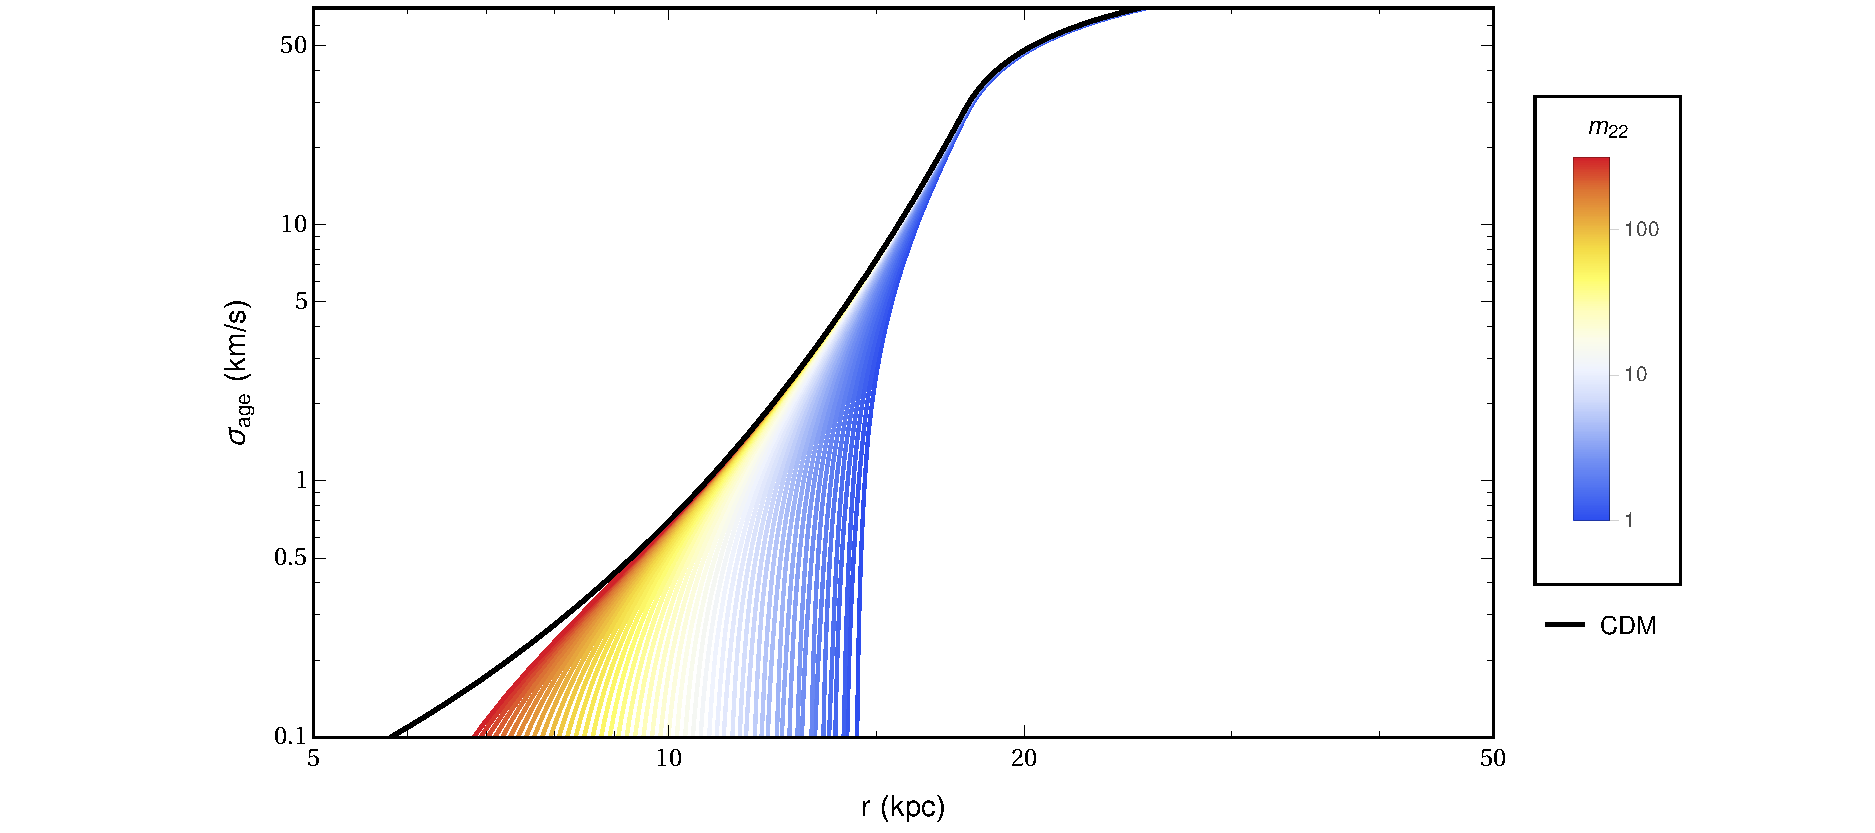
\includegraphics[width= 10cm]{CDM_velocity}
\vspace*{-5mm}
\caption{Rate of heating due to dynamical subhalos as a function of radius for a Milky Way-like halo with $M_p = 10^{12} \, M_\odot$ and $\Sigma_0 = 64 \, M_\odot \, \si{\per\parsec^2}$. The heating is calculated for subhalos in CDM and FDM with $m_{22} = 1$ respectively.}
\label{fig:CDMheating}
\end{figure}


\subsection{Heating in the FDM Paradigm}

\subsubsection{The Subhalo Mass Function}

The fluctuations due to subhalos dynamics are reduced in FDM compared to CDM because the halo mass function is suppressed at low mass due to the quantum Jeans scale. The FDM halo mass function is calculated numerically from the Press--Schechter formalism \citep{substructure_FDM, marsh} and the soliton profile is fitted from simulations by \cite{schive_solitons}. 


\subsubsection{Tidal Disruption}

We employ an identical method for truncating subhalos due to the tidal stripping of the primary halo. However, in FDM, light subhalos are more easily tidally disrupted via a runaway soliton reformation effect. If the tidal radius of a subhalo lies within its soliton core then mass from the soliton will be stripped away which, due to the self-gravitating quantum condition,
\begin{equation}
R \approx \frac{\hbar^2}{m_p^2 M G}
\end{equation} 
forces the soliton to grow in size causing a runaway effect which completely destroys the subhalo. This only requires us to modify our truncation function by setting $T_R(m) = 0$ if the tidal radius lies within the soliton radius. We can now compare the heating due to subhalos in the FDM and CDM paradigms and a function of the particle mass. The results are summarized in table \eqref{FDM_ratio}.   

\begin{table} \label{FDM_ratio}
\begin{center}
 \begin{tabular}{||c c||} 
 \hline
 $m_{22}$ & $\left( \frac{\sigma_{FDM}^2}{\sigma_{CDM}^2} \right)^{\tfrac{1}{2}}$ \\ [2.5ex] 
 \hline\hline
 0.75 & 0.140 \\ 
 \hline
 1.00 & 0.209 \\
 \hline
 1.50 & 0.257 \\
 \hline
 2.00 & 0.274 \\
 \hline
 3.00 & 0.701 \\
 \hline
 4.00 & 0.838 \\
 \hline
 5.00 & 0.896 \\
 \hline
 10.00 & 0.976 \\ [1ex] 
 \hline
\end{tabular}
\end{center}
\caption{The ratio of heating due to FDM subhalos and heating due to CDM subhalos at the solar neighborhood $R_0 = \SI{8}{\kilo\parsec}$ as a function of particle mass $m = m_{22} \cdot \SI{e-22}{\electronvolt}$. }
\end{table}

\begin{figure*}
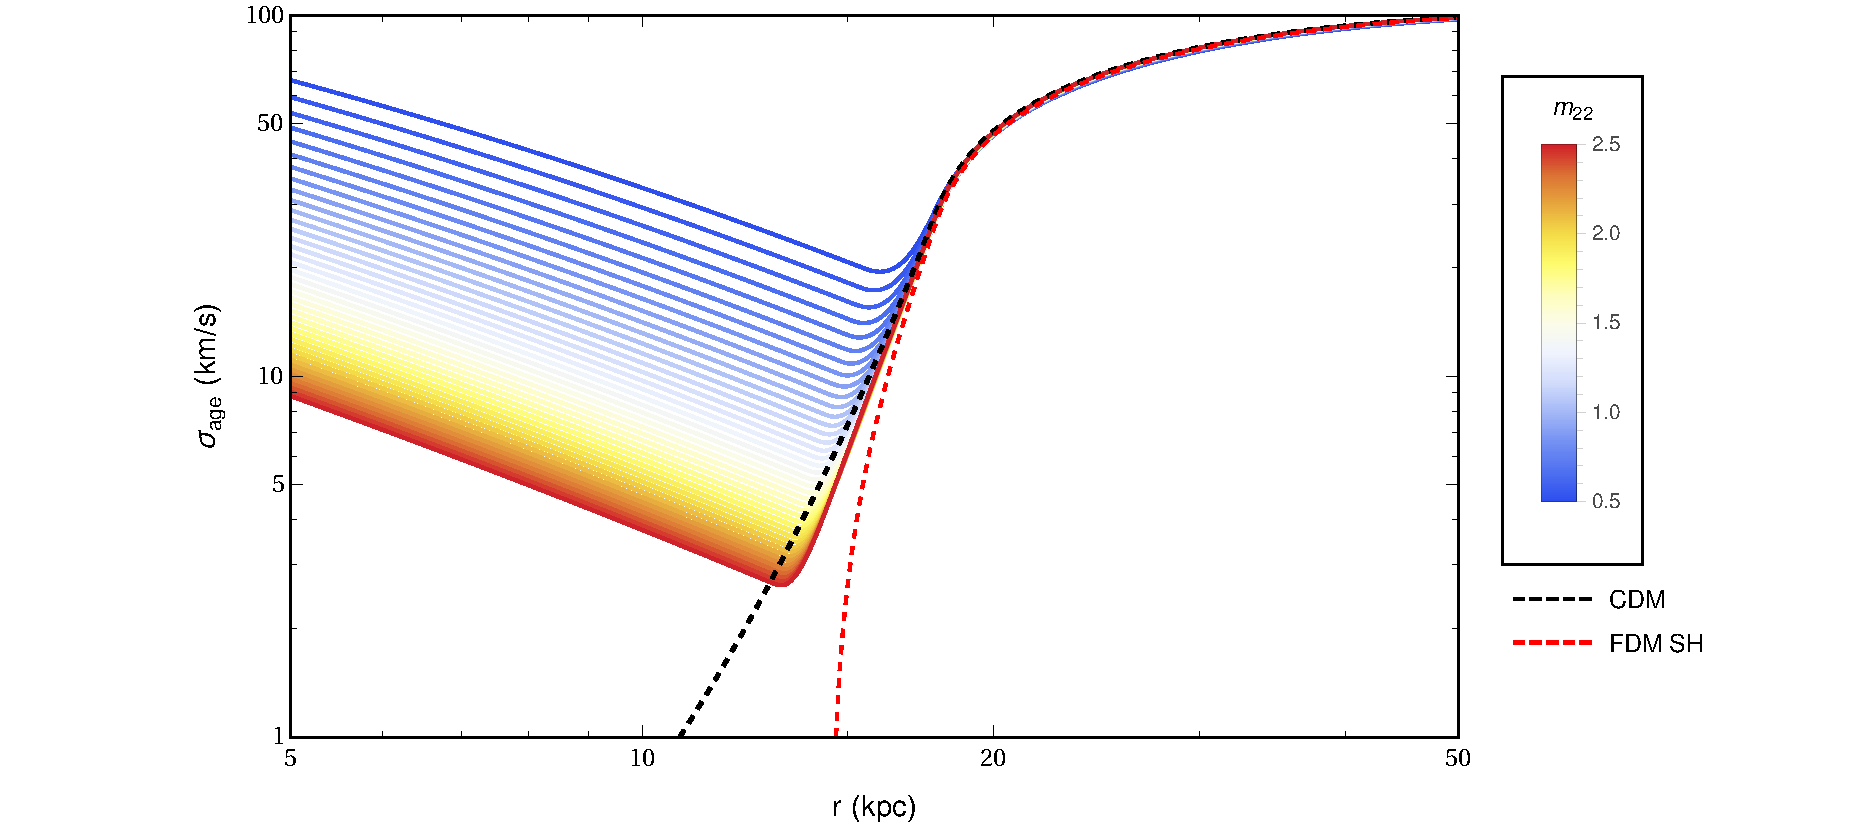
\includegraphics[width=17cm]{FDM_velocity}
\caption{Total Rate of heating due to FDM wavelets and subhalos as a function of radius for axion masses $m_{a}$ in the range \SIrange{0.25 e-22}{ 1.75 e-22}{\electronvolt}. for a Milky Way-like halo with $M_p = 10^{12} \, M_\odot$ and $\Sigma_0 = 64 \, M_\odot \, \si{\per\parsec^2}$. Dashed lines give the heating to subhalos alone in the CDM and FDM models (with $m_{22} = 1$) respectively.}
\label{fig:radiusheating}
\end{figure*}

\begin{figure}
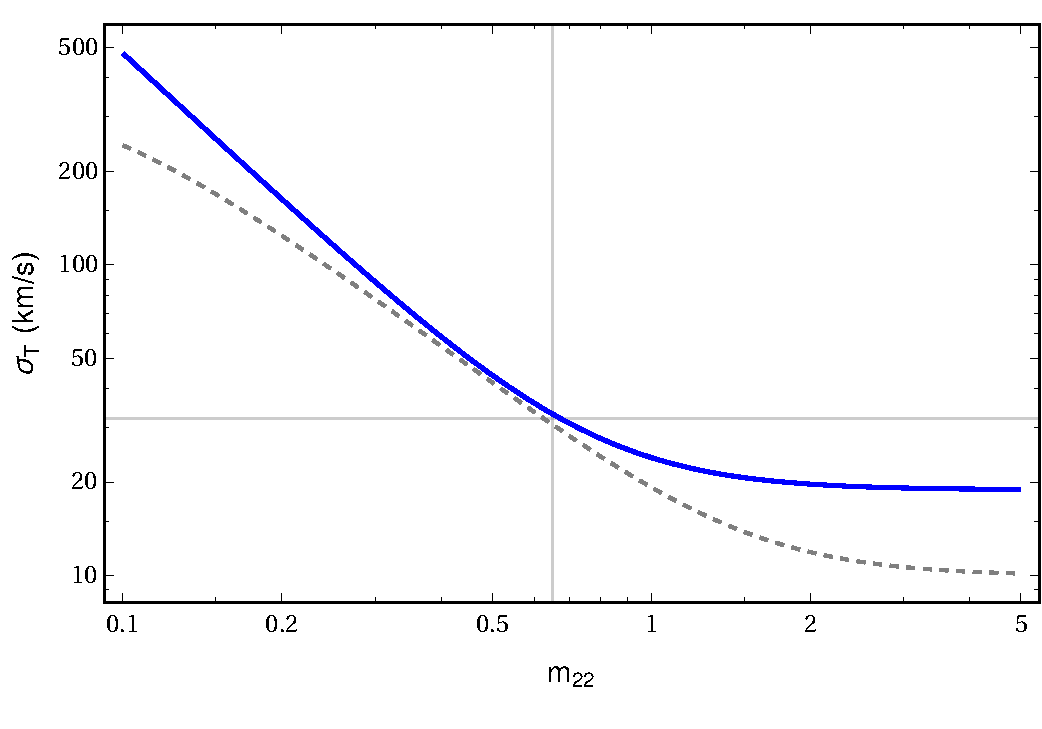
\includegraphics[width=\columnwidth]{FDM_mass_dep}
\vspace*{-5mm}
\caption{Rate of heating due to wavelets at $r = 8\, \si{\kilo \parsec}$ as a function of axion masses $m_{a}$ in the range \SIrange{0.1 e-22}{ 10 e-22}{\electronvolt}. for a Milky Way-like halo with $M_p = 10^{12} \, M_\odot$ and $\Sigma_0 = 64 \, M_\odot \, \si{\per\parsec^2}$. The horizontal line is fixed at $34\, \si{\kilo\meter\per\second}$, the observational maximum on velocity dispersion of the Milky Way thick disk. }
\label{fig:mass_dep_heating}
\end{figure}


\subsubsection{Fluctuations due to Wavelets}

Although the fluctuations due to subhalo transits are reduced in the FDM paradigm in comparison to CDM, for a moderately light particle mass ($m_p \approx \SI{e-22}{\electronvolt}$) the dominant effect is due to wavelets, the interference fringes produced by standing FDM waves. In the limit of large particle mass, FDM recreates the results of CDM since the subhalos act identically and the power in wavelets is strongly suppressed by a factor of $m_{22}^{-3}$. For very low particle masses, this power grows rapidly and easily exceeds observational bounds for the velocity dispersion of the Milky Way thick disk. We are primarily interested in the intermediate region in which the transition from wavelet dominated fluctuations to subhalo dominated fluctuations occurs. Figure \ref{fig:radiusheating} illustrates that the transition from wavelet dominated heating to subhalo dominated heating occurs approximately at $r \approx \SI{20}{\kilo \parsec}$. For large particle mass, $m_{22} \approx \SI{2.5e-22}{\electronvolt}$, the minimal heating occurs at $r \approx \SI{10}{\kilo \parsec}$. The radius of the minimal heating increases with decreasing particle mass. Furthermore, as the particle mass decreases, the transition between the wavelet dominated and subhalo dominated regimes becomes smoother and the minimum between the two regimes is ameliorated.   


\begin{table} \label{FDM_ratio}
\begin{center}
 \begin{tabular}{||c c c||} 
 \hline
 $m_{22}$ & $A^{-\tfrac{1}{2}} \left( \frac{\sigma_{W}^2}{\sigma_{SH}^2} \right)^{\tfrac{1}{2}}$ & $ \left( \frac{\sigma_{W}^2}{\sigma_{SH}^2} \right)^{\tfrac{1}{2}} \bigg|_{A = 2.2}$ \\ [2.5ex] 
 \hline\hline
 0.75 & 48.03 & 71.25 \\ 
 \hline
 1.00 & 21.85 & 32.42 \\
 \hline
 1.50 & 10.26 & 15.22 \\
 \hline
 2.00 & 6.47 & 9.60 \\
 \hline
 3.00 & 1.45 & 2.14 \\
 \hline
 4.00 & 0.81 & 1.20 \\
 \hline
 5.00 & 0.55 & 0.82 \\
 \hline
 10.00 & 0.19 & 0.29 \\ [1ex] 
 \hline
\end{tabular}
\end{center}
\caption{The ratio of heating due to FDM wavelets and heating due to FDM subhalos at the solar neighborhood $R_0 = \SI{8}{\kilo\parsec}$ as a function of particle mass $m = m_{22} \cdot \SI{e-22}{\electronvolt}$. The values are quoted both as a function of the amplitude $A$ and for the value $A = 2.2$. }
\end{table}

\section{Conclusion}

\begin{figure*}
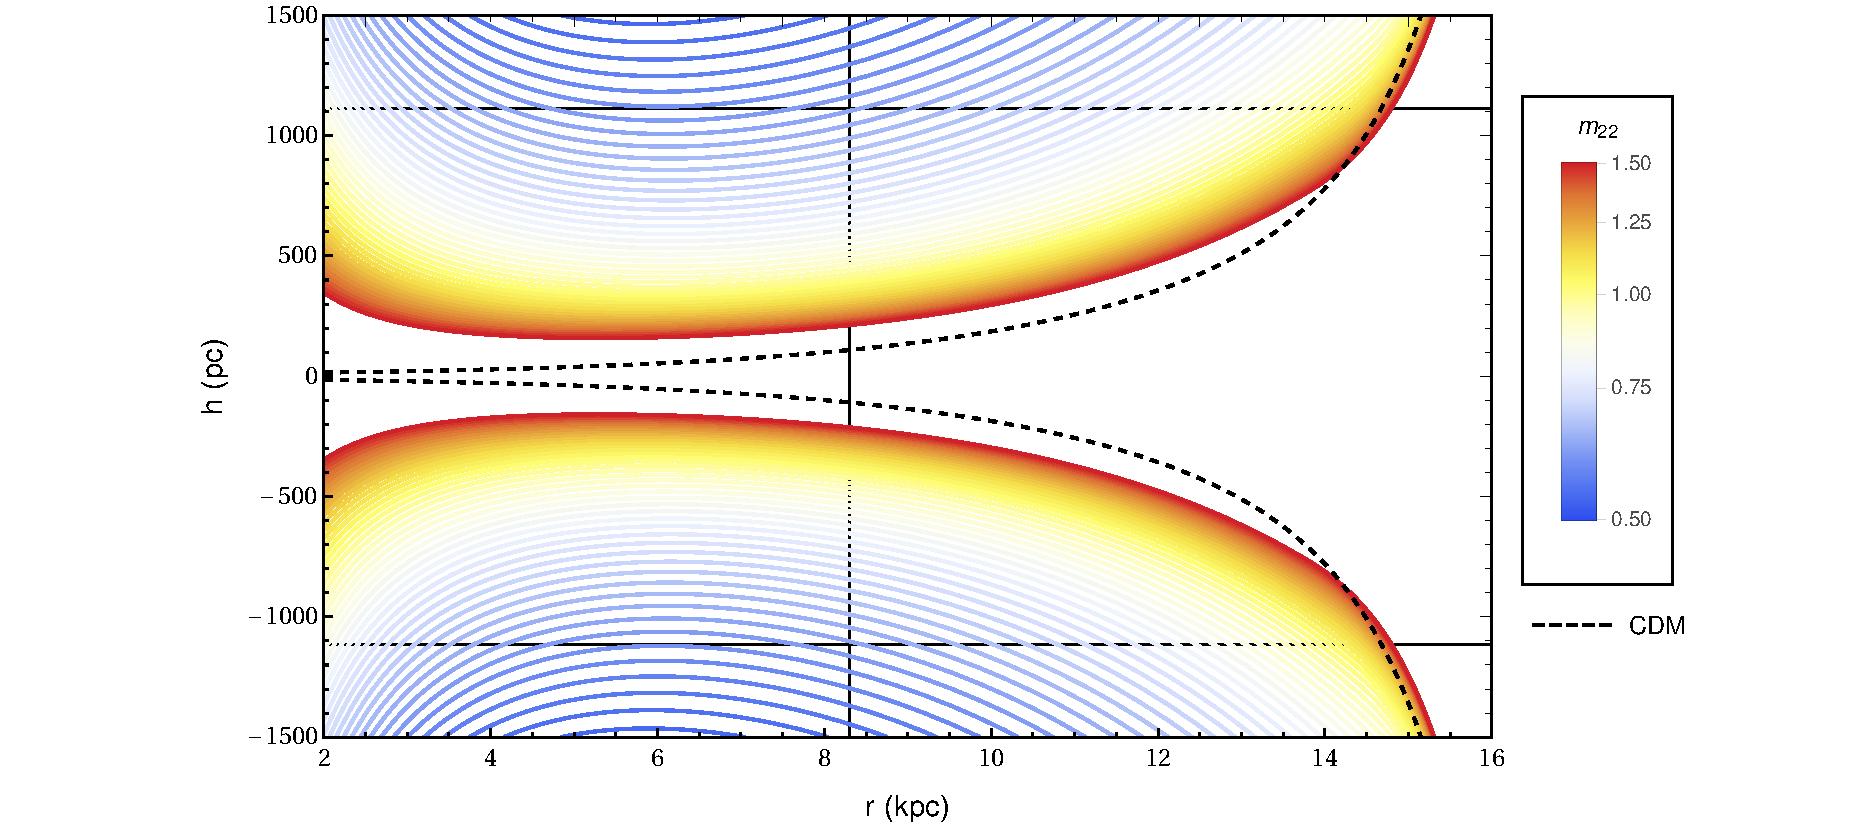
\includegraphics[width=18cm]{disk_shape}
\vspace*{-5mm}
\caption{Profile of the galactic disk thickness induced by substructure heating as a function of radius for a Milky Way-like halo with $M_p = 10^{12} \, M_\odot$ and $\Sigma_0 = 64 \, M_\odot \, \si{\per\parsec^2}$. The velocity dispersion of the disk is assumed to be entirely produced by heating due to FDM wavelets. }
\label{fig:disk_shape_FDM}
\end{figure*}

\subsection{Disk Destruction at Large Radii}

Given a dark matter paradigm, we have shown how to estimate the heating of the disk caused by dynamical substructure. If we make the further assumption that dark substructure is the dominant disk thickening effect then we have a method of predicting the actual velocity dispersion of a disk as a function of radius. However, in a galaxy with a known surface density   profile, there is a simple relationship between the velocity dispersion and the scale height of a disk given by equation \eqref{scale}. Therefore, we can compare the disk shapes predicted by CDM and FDM shown in figure \ref{fig:disk_shape_FDM} respectively. Subhalos alone cause very little thickening out to a radius of approximately $\SI{15}{\kilo \parsec}$ at which point the disk flares exponentially. This rapid growth in thickness will cause the outer disk to become unstable and lead to disk destruction beyond a certain radius. 
\par 
We consider two possible criteria to determine the point at which a galactic disk is destroyed by thickening. The first naive criterion is that, 
\begin{equation}
\frac{H(r)}{r} > 1
\end{equation}
This clearly gives an upper bound on the endpoint of the disk. Using this criterion, if the disk is thickened by CDM subhalos alone then the disk will be destroyed past a radius at most $r = \SI{18.5}{\kilo \parsec}$ (see figure \ref{fig:disk_shape_FDM}). Figure \ref{fig:disk_shape_FDM} shows that the disk shape is not highly sensitive to particle mass and therefore to the total rate of heating. Therefore, CDM and FDM paradigms do not significantly differ in predicting disk destruction beyond a radius of $r = \SI{18.5}{\kilo \parsec}$. In fact, the disk flare is mostly determined by density profile of the disk itself.  
\par
Here, we propose a more sensitive condition for the point of disk destruction. We will call a disk destroyed if stars with large vertical displacements are bound by the dark matter halo rather than the gravity due to the disk surface density. Therefore, we require that,
\begin{equation}
\frac{M(r) G}{r^2} = \frac{v_c^2}{r} > 4 \pi G \Sigma(r) 
\end{equation}   
This condition is purely geometrical and surprisingly independent of the disk heating. However, we find that for a Milky Way-like halo with $M = 10^{12} M_{\odot}$ and $\Sigma_0 = \SI{64}{M_{\odot} \per \parsec \squared}$ that this condition is always satisfied. 
\par
FDM wavelets on the other-hand can produce significant thickening at all radii. For example, at the solar neighborhood $R_0$ an axion of mass $m_p = \SI{1.3 e-22}{\electronvolt}$ will lead to a scale height of $\SI{1.6}{ \kilo\parsec}$ if both disk heating processes are effective. If only the lower bound given by tidal effects is allowed then the time scale over which significant disk thickening occurs is much longer than the current age of the universe \citep{ultralight}. Wavelets will also give rise to exponentially flaring disks. However, because wavelets produce their maximum power at small radii and subhalos at large radii, the disk flaring caused by wavelets is significantly weaker than the CDM counterpart. Furthermore, the transition point from an approximately flat disk to a flaring disk is highly sensitive to particle mass. Therefore, the radius at which disk destruction takes place is quite sensitive to $m_{22}$ although it will be at a larger radii than then comparable CDM number because there are fewer low mass subhalos predicted by FDM than by CDM. 


\subsection{Constraints on Particle Mass}

The Milky Way disk has two components, a recently formed thin disk with low velocity dispersion and a old thick disk with large relatively large velocity dispersion. The thick disk has locally a velocity dispersion of approximately \SI{34}{\kilo\meter\per\second} in its thickest parts \citep{milky_way}. Therefore, the velocity dispersion caused by substructure heating cannot exceed this value. We find that CDM does not produce sufficient heating to be constrained by observational measurements of the local  Milky Way disk. However, the heating due to wavelets in FDM is strongly dependent on particle mass and far more efficient than other substructure. In the low-mass limit, the heating may vastly exceed observational bounds. Using the results quoted for the velocity dispersion of the thick disk as a strict cutoff, we derive a lower bound on the mass of the FDM particle,
\begin{equation}
m_p > 0.94 A^{1/3} \times \SI{e-22}{\electronvolt}
\end{equation}
Using the best estimate of $A \approx 2.2$, we obtain the most probable lower bound on the FDM particle mass of,
\[ m_p > 1.27 \times \SI{e-22}{\electronvolt} \]
under the assumption that all disk heating is reflected in the z-velocity dispersion.
\par
One source of contention between our theoretical treatment and observation is our prediction for the heating history of the disk. Both dark matter paradigms predict a constant rate of heating independent of the velocity dispersion of the disk and therefore a time dependent velocity dispersion $\sigma_D \approx t^{\beta}$ with $\beta = \tfrac{1}{2}$. This disagrees with observations which suggest that the Milky Way thick disk has increased in velocity dispersion with exponent $\beta \approx \tfrac{1}{3}$ \citep{heating_history}. However, these calculations assume that dark substructure alone (ignoring, for example, the contribution due to spiral structure heating effective at low values of $\sigma$) is responsible for disk heating. Multiple sources of heating may combine to produce a lower effective exponent. 


\subsection{Summary}
We find that the heating of Milky Way type stellar disks by subhalo gravitational fluctuations will lead to flaring and disk destruction at radii greater than 15-\SI{20}{\kilo\parsec} in both CDM and FDM paradigms. However, quantum wavelets in FDM can be effective at heating the inner disk regions. A particle mass in excess of $m_p \approx \SI{1.27 e-22}{\electronvolt}$ is required to avoid exceeding observational bounds on heating of thick disk stars in the Milky Way. Correspondingly, an FDM scenario with particle mass $m_p \approx 1-\SI{2e-22}{\electronvolt}$ can, in fact, explain the observed increase in velocity dispersion with increasing stellar age observed in the solar neighborhood.    


\section*{Acknowledgments}
We thank Mihir Kulakarni for his code to calculate the FDM halo mass function and his invaluable guidance on this project. We further thank Hsi-Yu Schive for helpful discussions on the nature of FDM solitons and wavelets. Many thanks to Scott Tremaie for his helpful critism and insights regarding the transfer of energy to disk thickening from bending modes of the disk vesus tidal strain. Support (PM) for this work was provided by NASA through the Einstein Postdoctoral Fellowship grant no. PF7-180164 awarded by the Chandra X-ray Center which is operated by the Smithsonian Astrophysical Observatory for NASA under contract NAS8-03060. 

\bibliography{mybib}


 
\end{document}
